% LaTeX file for Chapter 02


\chapter{Methods}

\section{Alignment and quantification with \emph{alevin-fry}}
\emph{Alevin} was developed to tackle the computational challenges that come with scRNA-seq data and to provide a tool that supports technologies other than 10x Genomics. \emph{Alevin} works in two steps. First, it parses a read file which contains the cellular barcode and a unique molecule identifier to generate a frequency distribution of observed barcodes. Second, it maps the reads to the transcriptome and generates a cell-by-gene count matrix. \emph{Alevin-fry} \citep{alevin_fry} was designed to be the successor to alevin and achieves similar accuracy at significantly lower computational costs. It generates a permit list for cellular barcodes that will be quantified in subsequent steps. By using a multi-thread approach, \emph{alevin-fry} filters and collates the mapping records for permitted cellular barcodes to produce a representation optimized for quantification \citep{alevin_fry}. We use \emph{alevin} and \emph{alevin-fry} for our analyses, in particular we focus on \emph{alevin-fry} as it outputs unspliced, spliced and ambiguous (USA) counts and equivalence classes (EC) that are required by the approaches we propose (i.e. USA counts for \emph{DEXSeq} and ECs for \emph{DifferentialRegulation}).

\begin{figure}[!htb]
\begin{center}
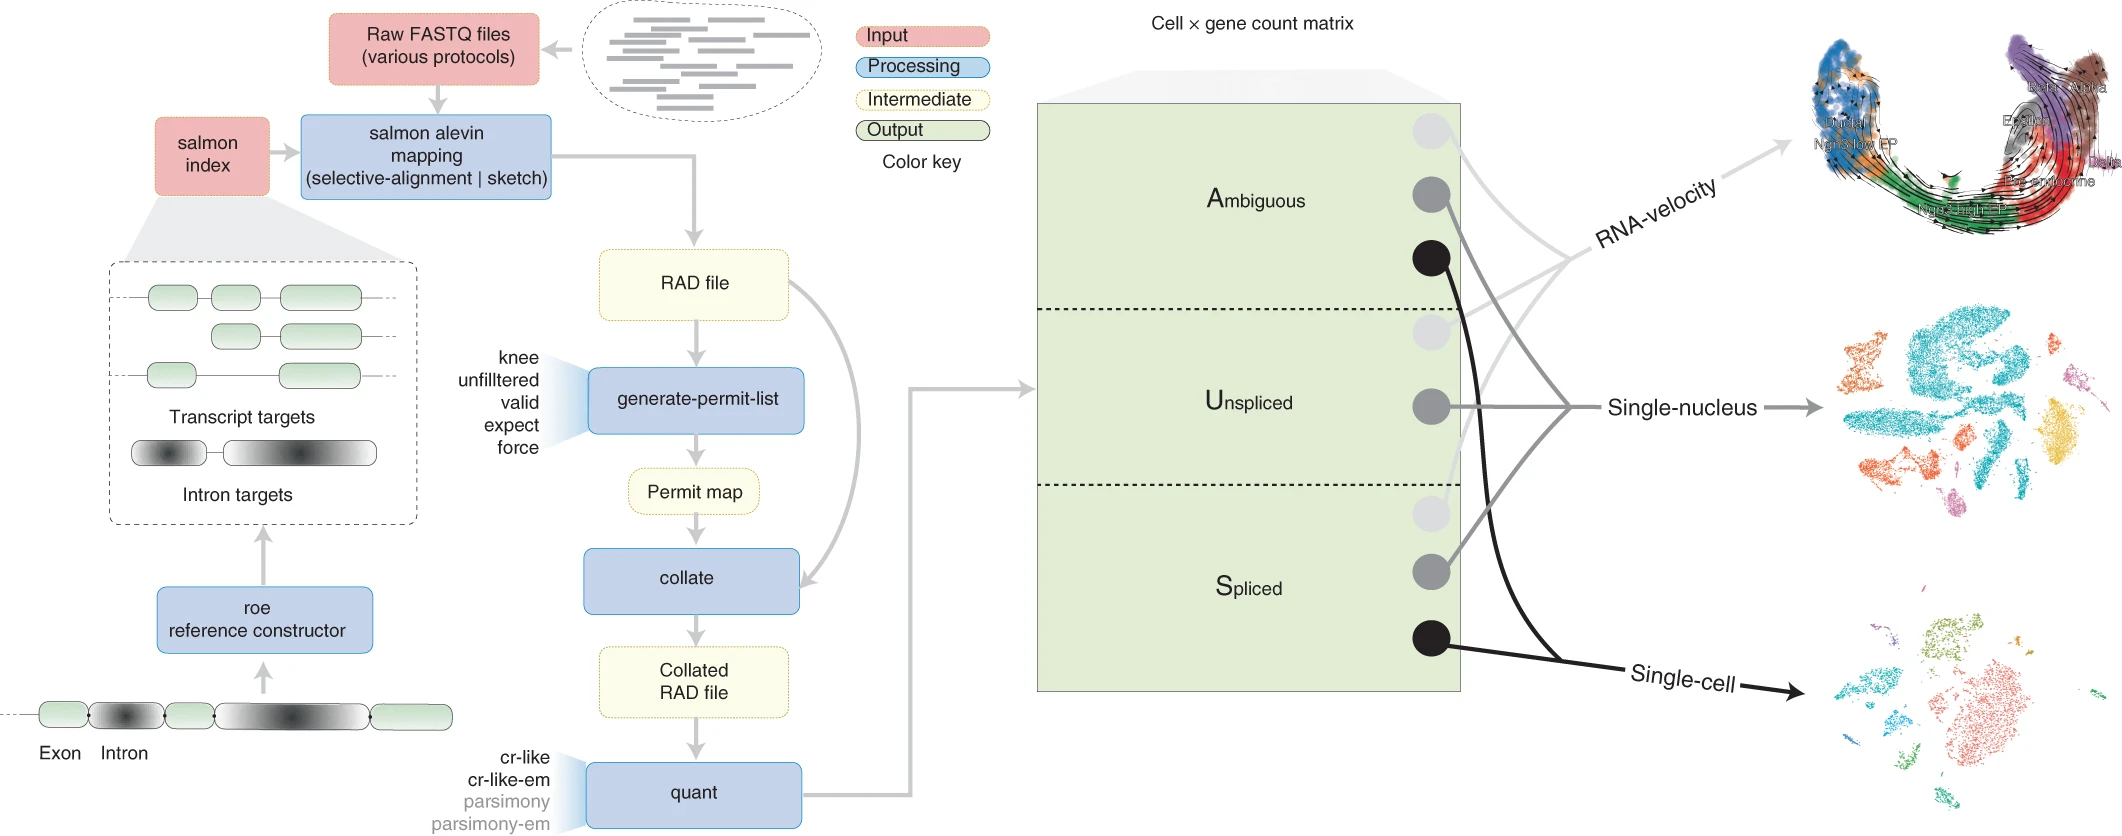
\includegraphics[width=6in,height=3in]{../figures/alevin_fry_pipeline.png}
\end{center}
\caption{Visualization of the \emph{alvein-fry} pipeline from start to finish \citep{alevin_fry}}
\label{fig:alevin_fry_pipeline}
\end{figure}
\FloatBarrier

\section{Read-level simulation with minnow}
\emph{minnow} is a read level simulator for droplet based scRNA-seq data that accounts for important sequence-level characteristics and model effects \citep{minnow}. It matches the gene-level ambiguity characteristics that are present in real scRNA-seq experiments. With \emph{minnow} it is possible to demonstrate the effect of gene-level sequence ambiguity on accurate quantification, which is used in this thesis to simulate mapping uncertainty between spliced and unspliced counts. It achieves this by either simulating sequences from the underlying de-Bruijn graph of the reference transcriptome or from the reference transcriptome directly \citep{minnow}. The \emph{minnow} framework essentially works in three steps: (i) selection of transcript, (ii) simulation of cell barcode (CB) and unique molecular identifier (UMI) tagging and (iii) simulation of polymerase chain reaction (PCR), fragmentation and sequencing. PCR is a laboratory technique to rapidly produce millions of copies of a specific DNA segment \citep{pcr}. First, \emph{minnow} uses a gene-count matrix as input that provides an estimated number of distinct molecules corresponding to each gene and cell in the sample. \emph{minnow} treats the normalized values of a particular cell as a multinomial distribution, then samples such molecules from that distribution \citep{minnow}. Figure \ref{fig:minnow_process} illustrates the process from input to simulated reads. \emph{Minnow} is used in this thesis to simulate at the read-level, which are afterwards aligned and quantified with \emph{alevin-fry}. This leads to a realistic simulation, which incorporates multi-mapping uncertainty, whose modelling is the primary objective of this thesis.

\begin{figure}[!htb]
\begin{center}
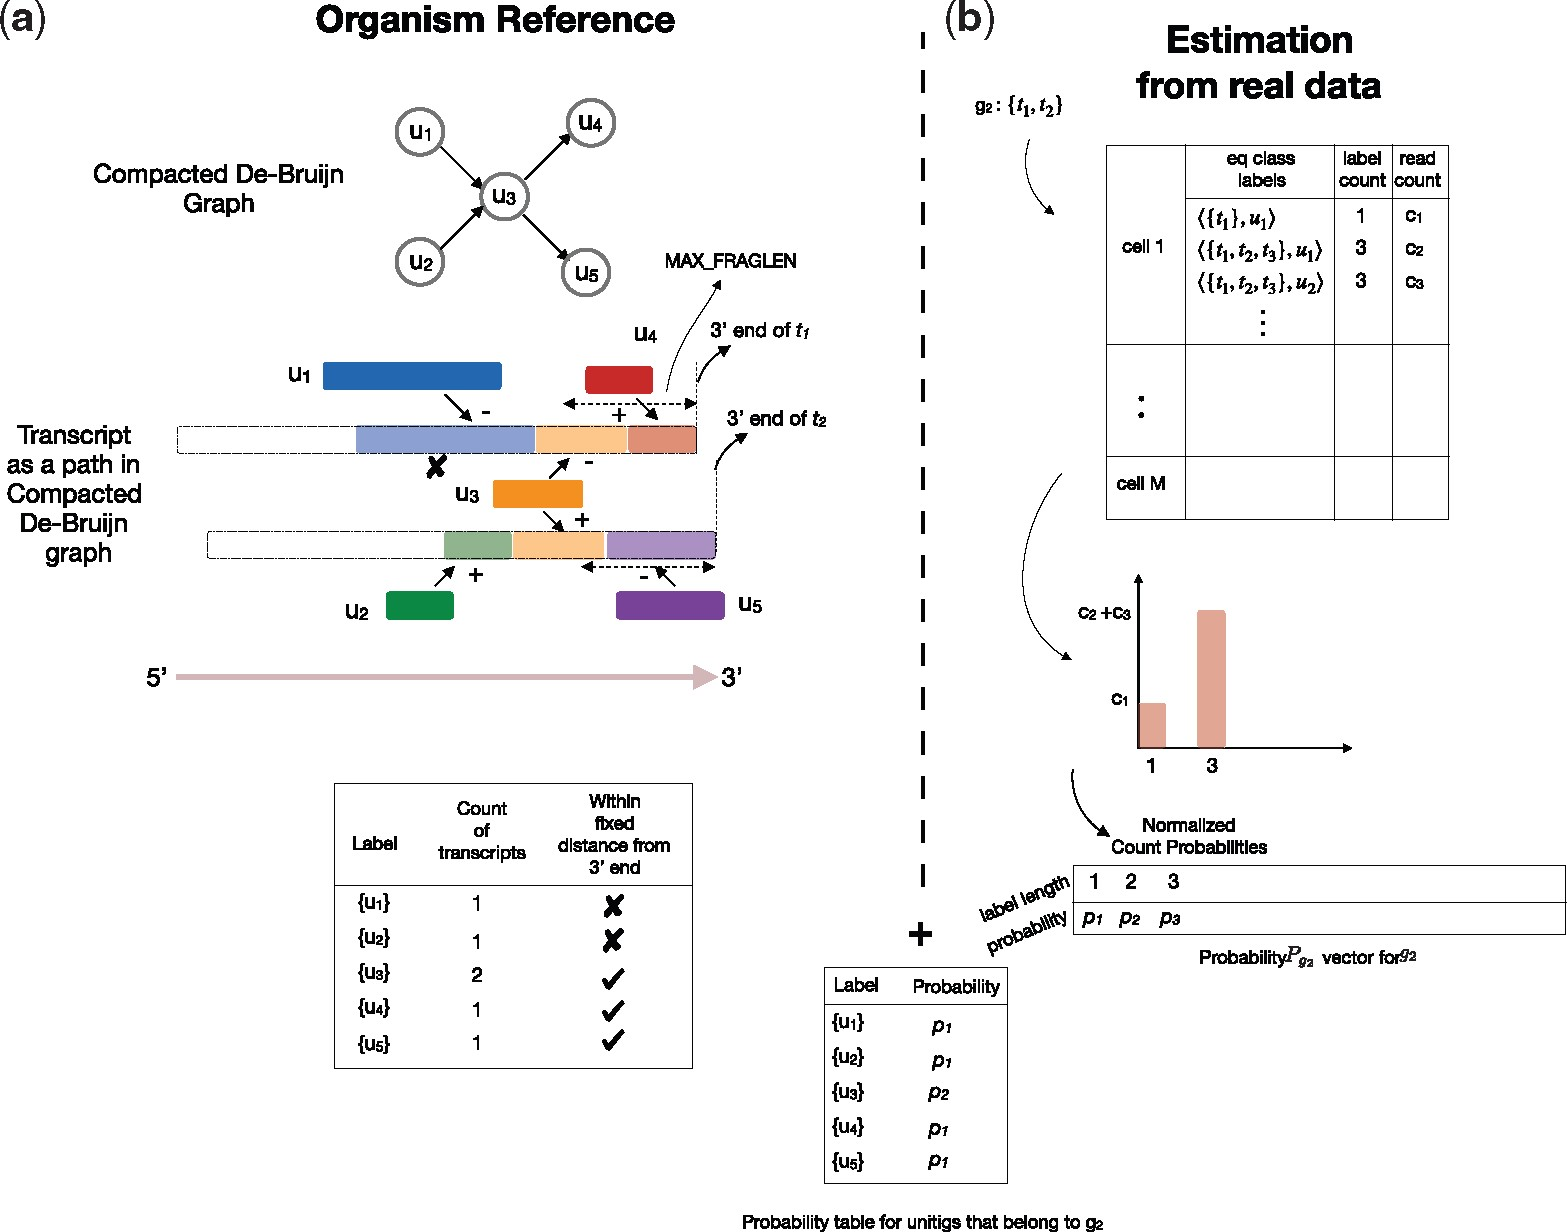
\includegraphics[width=6in,height=4in]{../figures/simulation/minnow_process.jpg}
\end{center}
\caption{Summary of the two possible pathways of \emph{minnow} from start to simulated reads \citep{minnow}}
\label{fig:minnow_process}
\end{figure}
\FloatBarrier

\section{Differential methods}
\subsection{\emph{eisaR}}
Exon-intron split analysis (EISA) is a computational approach that measures mature RNA and pre-mRNA reads across different experimental conditions \citep{eisar}. The method has been developed to quantify transcriptional and post-transcriptional regulation of gene expression. After quantification of exonic and intronic reads, both counts are normalized to the mean library size and $log_2$-transformed with the addition of a pseudocount of 8. Based on these expression levels, very lowly expressed genes (average $log_2$ expression of at least 5) in either exons and introns are removed, such that there is a fixed set of quantifiable genes. As absolute exonic and intronic counts have very different distributions it is difficult to model them in the same statistical model \citep{eisar}. Therefore, the difference of $\Delta \text{exon}$ and $\Delta \text{intron}$ is modelled with a generalized linear regression model to mitigate this issue. The generalized linear regression approach uses an interaction term to determine the statistical significance between exonic and intronic counts and the experimental conditions, and is implemented within the \emph{edgeR} framework \citep{edger_package} that is used to examine differential gene expression of replicated count data where the counts are modelled by a negative binomial distribution (\ref{eqn:edger}), where for the \emph{g}-th gene and \emph{i}-th sample:

\begin{equation}
Y_{gi} \sim NB(\text{mean} = M_{i}\rho_{gj}, \text{dispersion} = \phi_g)
\label{eqn:edger}
\end{equation}

where $M_i$ is the library size (total counts) for i-th sample; $\phi_g$ is the dispersion for the g-th gene and $\rho_{gj}$ is the relative abundance of gene g in experimental group j which sample i belongs to and $\text{NB(a, b)}$ denotes the negative binomial distribution with mean a and dispersion b. Ultimately, the significance of the interaction term is calculated by the use of a likelihood ratio test between the full model and a reduced model containing the experimental condition without the interaction term \citep{eisar}. In this thesis we used the R package \emph{eisaR} which implements the EISA framework to conveniently run the method \citep{eisar_package}.

\subsection{\emph{BRIE2}}
\emph{BRIE2} is a scalable computational method that regresses single-cell RNA-seq data against cell-level features \citep{brie2}. Unavoidable difficulty in the quantification arises from the fundamental ambiguity of the data, because a majority of reads cannot be mapped unambiguously to a single isoform. \emph{BRIE1} tackled this issue by regressing percentage of spliced-in (PSI) values through a Bayesian regression approach. However, \emph{BRIE1} is not well suited to quantify differential splicing across cell types because sequence features are usually the same between individual cells \citep{brie2}. \emph{BRIE2} again starts from a latent regression framework, however, it differs from \emph{BRIE1} in two important ways: first, it augments the set of regressor features by including cell-specific information e.g. cell type; second, the added complexity considerably increases the computational cost. Therefore, because of its elevated computational complexity, \emph{BRIE2} was developed to be used in conjunction with advanced software e.g. Tensorflow and graphics processing units (GPUs), which significantly increases computational acceleration. Figure \ref{fig:brie2_process} summarizes the process from input to output in the \emph{BRIE2} pipeline.

The BRIE2 model uses a generalised linear model to identify regulatory factors of splicing from both gene and cell level features \citep{brie2}. It assumes that $z_{c,g}$ is a linear combination as follows:

\begin{equation}
z_{c,g} = \alpha_c^T x_g + y_c^T \beta_g + \epsilon_{c,g}
\label{eqn:brie_A}
\end{equation}

where $x$ denotes the gene level features and $y$ denotes the cell level features; $\alpha_c^T$ is the gene specific and $\beta_g$ is the cell feature specific coefficient. In this thesis we use \emph{BRIE2} in the differential momentum genes mode, which allows the detection of differential alternative splicing events or differential momentum genes with one or multiple cell-level covariates \citep{brie2}. This is equivalent to selecting model 1 ($M_1$) with significant effects against model 0 ($M_0$) with no effects.

\begin{equation}
M_0: p_g^{(0)} = \prod_{c=1}^{M}{p(s_{c,g} | z_{c,g}) N(z_{c,g} | y_{c,t} \cdot 0 + y_{c,t^-}^T \beta_{g,t^-}, \sigma_g^2)}
\label{eqn:brie_B}
\end{equation}

\begin{equation}
M_1: p_g^{(1)} = \prod_{c=1}^{M}{p(s_{c,g} | z_{c,g}) N(z_{c,g} | y_{c,t} \cdot \beta_{g,t} + y_{c,t^-}^T \beta_{g,t^-}, \sigma_g^2)}
\label{eqn:brie_C}
\end{equation}

where $N(a,b)$ is the normal distribution with mean $a$ and variance $b$; $t^-$ denotes all cell features except feature t; $p(s_{c,g} | z_{c,g})$ is the multinominal, conditional distribution given $z_{c,g}$ where $s_{c,g}$ is the three dimensional count vector.

\begin{figure}[!htb]
\begin{center}
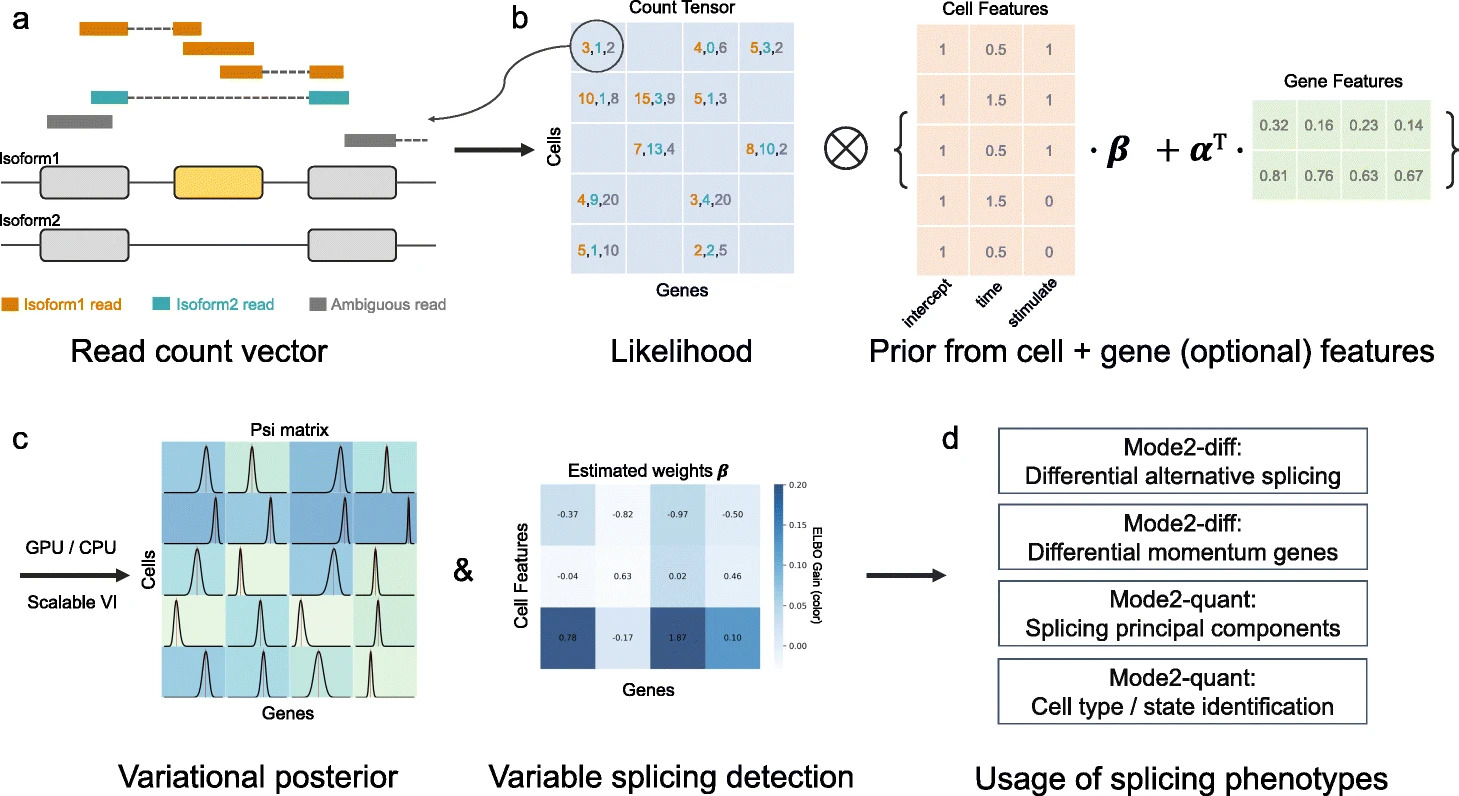
\includegraphics[width=6in,height=3in]{../figures/brie2_process.jpg}
\end{center}
\caption{Summary of the estimation process of \emph{BRIE2} \citep{brie2}}
\label{fig:brie2_process}
\end{figure}
\FloatBarrier

\subsection{\emph{DEXSeq}}
\emph{DEXSeq} \citep{dexseq} is a statistical method originally proposed to test for differential exon usage in RNA- seq data, which has been widely adopted in other contexts too, such as differential transcript usage \citep{swimming_downstream}. The model is based on the negative binomial distribution and allows for covariates such as batch effects to be taken into account to offer reliable control of false discoveries \citep{dexseq}. In its original implementation \emph{DEXSeq} inputs how many reads map to each exon, but the method has also been used on transcript level counts [\citep{swimming_downstream}, \citep{bandits}]. Equation (\ref{eqn:DEXSEQ_A}) shows that the read counts follow a negative binomial distribution where $\alpha$ is the dispersion parameter. Further, a generalized linear model is used to predict the mean via a log-linear link, where for gene \emph{i}, exon \emph{l} and sample \emph{j}:

\begin{equation}
K_{ijl} \sim \text{NB}(\text{mean}=s_j \mu_{ijl}, \text{dispersion}=\alpha_{il})
\label{eqn:DEXSEQ_A}
\end{equation}

\begin{equation}
log(\mu_{ijl}) = \beta^G_i + \beta^E_{il} + \beta_{i \rho_j}^C + \beta^{EC}_{i \rho_j l}
\label{eqn:DEXSEQ_B}
\end{equation}

where $\text{NB(a, b)}$ denotes the negative binomial distribution with mean a and dispersion b, $\alpha_{il}$ is the dispersion parameter; $s_j$ is the size factor for the \emph{j}-th sample; $\mu_{ijl}$ is the expected value of the concentration of cDNA fragments of the \emph{l}-th exon of \emph{i}-th gene in sample \emph{j}; $\rho_j$ is the group sample \emph{j} belongs to; $\beta^G_i$ is the baseline expression strength of gene \emph{i}; $\beta^E_{il}$ is the coefficient for the \emph{l}-th exon in gene \emph{i}; $\beta^C_{i\rho_j}$ is the coefficient for the group $\rho_j$ in gene \emph{i}; $\beta^{EC}_{i \rho_j l}$ is the exon-condition interaction term for condition $\rho_j$ and exon \emph{l} in gene \emph{i}.

The dispersion parameter allows to model over-dispersed data (i.e. higher variance than mean). Here, we propose to use \emph{DEXSeq} on estimated USA counts, and perform a differential usage test between experimental conditions. Therefore, for every gene, exons are replaced by the spliced, unspliced and ambiguous versions of the gene. This models ambiguous reads separately from spliced and unspliced or exonic and intronic, thus eliminating one of the main sources of mapping uncertainty. However, the uncertainty related to reads mapping to multiple genes is still neglected by this approach. To address both sources of mapping uncertainty we propose a novel method, developed by Simone Tiberi \citep{differential_regulation}.

\subsection{\emph{DifferentialRegulation}}

\section{Analysis of results}
\subsection{Unifold Manifold Approximation and Projection (UMAP)}
Unifold Manifold Approximation and Projection (UMAP) is a dimension reduction technique that can be used to visualize data from a high-dimensional space into a low-dimensional space \citep{umap}. UMAP is implemented on the following three assumptions about the data: first, the data is uniformly distributed on the Riemannian manifold \citep{riemann}; second, the Riemannian metric is locally constant \citep{riemann}; third, the manifold is locally connected. Essentially, UMAP constructs a high dimensional graph representation of the data and then tries to fit a low-dimensional graph that is as structurally similar as possible \citep{umap}. In this thesis UMAP is used to assess how cells cluster i.e. based on their cell type or to which sample they belong. This knowledge is important, for example to evaluate whether there are structural differences between samples, although the samples are biological replicates. Figure \ref{fig:umap} shows the clustered digits of the famous MNIST data set which consists of 28x28 pixel grayscale images of handwritten digits (0 through 9) \citep{mnist}. Each digit is described by a 784 dimensional vector which hereby was reduced to a two-dimensional representation by applying UMAP.

\begin{figure}[!htb]
\begin{center}
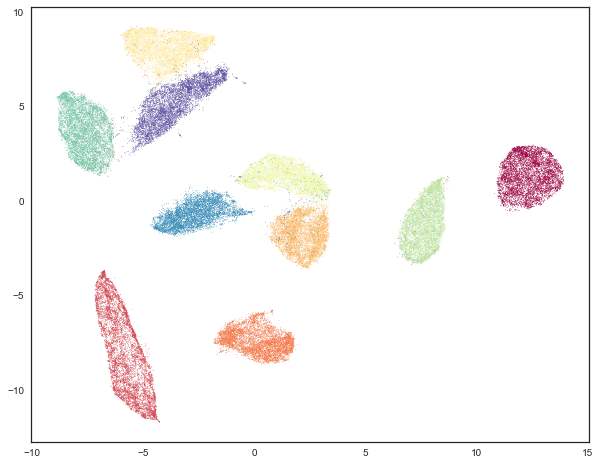
\includegraphics[width=6in,height=4in]{../figures/umap.png}
\end{center}
\caption{Example of a UMAP representation of high dimensional data into two dimensions highlighting the data clusters \citep{umap_implementation}}
\label{fig:umap}
\end{figure}
\FloatBarrier

\subsection{Classification measurements}
The true positive rate (TPR), false positive rate (FPR), and false discovery rate (FDR) are defined as:

\begin{equation}
\text{TPR}=\frac{|\text{TP}|}{|\text{TP}+\text{FN}|}
\label{eqn:tpr}
\end{equation}

\begin{equation}
\text{FPR}=\frac{|\text{FP}|}{|\text{FP}+\text{TN}|}
\label{eqn:fpr}
\end{equation}

\begin{equation}
\text{FDR}=\frac{|\text{FP}|}{|\text{TP}+\text{FP}|}
\label{eqn:fdr}
\end{equation}

where TP, TN, FP, and FN indicate the sets of true positive, true negative, false positive, and false negative elements, respectively. TP are the number of elements that were correctly identified as the positive outcome. Similarly, TN are the number of elements that were correctly identified as the negative outcome. FP are those elements that were identified as the positive outcome, however they should have been identified as negative. In statistics, FP is usually referred to as Type 1 error. Similarly, FN are the elements that were incorrectly identified as negative - also referred to as Type 2 error in the realms of statistics. Figure \ref{fig:confusion_matrix} illustrates the meaning of these measurements quite clearly. The TPR (true positive rate) also referred to as sensitivity, measures the proportion of positive elements that were correctly identified - often alluded to as statistical power (\ref{eqn:tpr}). The FPR (false positive rate) measures the proportion of negative outcomes that are identified as positive (\ref{eqn:fpr}). On the other hand, FDR (false discovery rate) measures the expected proportion of false positive among all positive predictions (\ref{eqn:fdr}). 

\begin{figure}[!htb]
\begin{center}
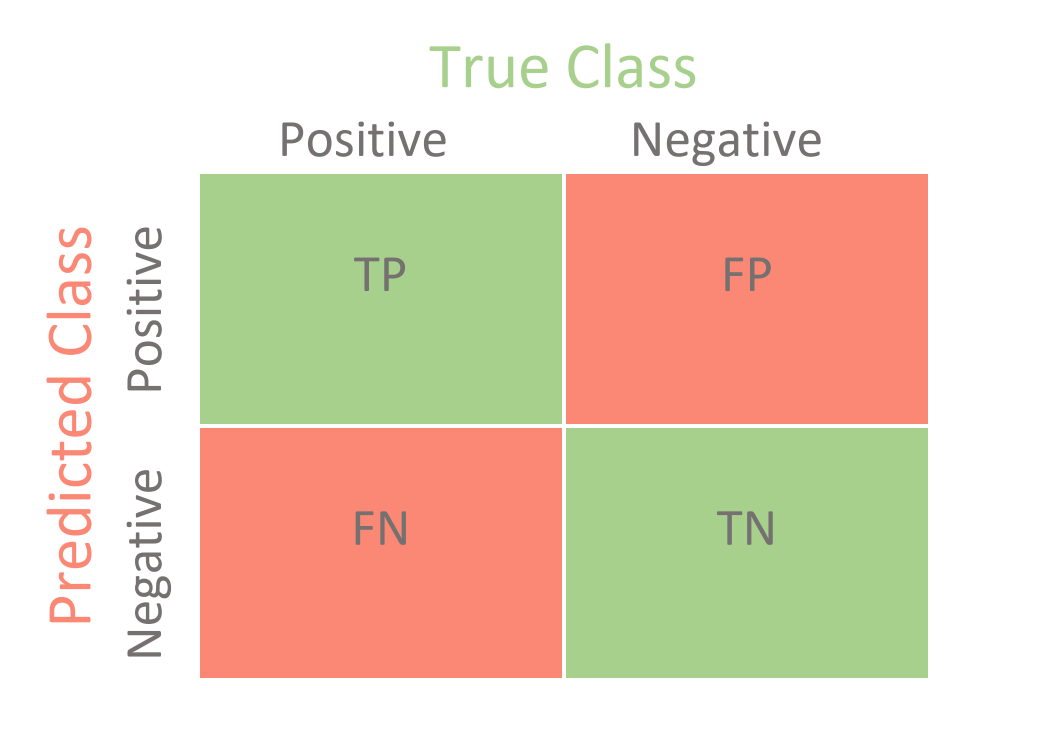
\includegraphics[width=6in,height=4in]{../figures/confusion_matrix.png}
\end{center}
\caption{Confusion matrix reporting the performance of a binary classification problem \citep{confusion_matrix}}
\label{fig:confusion_matrix}
\end{figure}
\FloatBarrier

\subsection{ROC curve}
The ROC curve is a performance measurement that is used for classification problems - in this case whether a gene is differently regulated or not. Essentially, the ROC curve plots the TPR (y-axis) against the FPR (x-axis). ROC curves above the diagonal indicate better performance than blind random guessing, denoted by the diagonal line. ROC curves are one of the performance evaluation methods used in this thesis.

\subsection{TPR v. FDR curves}
Similar to the ROC curve the TPR v. FDR curve is used to assess performance in classification problems. It plots the TPR (y-axis) against the FDR (x-axis). In addition, one often plots the actual which was observed for some theoretical thresholds - usually 1, 5 and 10\%. FDR values are essentially adjusted p-values which can be calculated in various ways from raw p-values. Arguably, the most popular one being the Benjamini-Hochberg correction \citep{BH_correction}. All the methods considered in this thesis, provide FDR adjusted p-values obtained via Benjamini-Hochberg correction.

When the observed FDR is lower than or equal to the specified threshold, the method controls for the FDR. However, if the observed FDR is greater than the threshold the method does not control for the FDR and there is an inflation of false positive predictions. In this thesis, the methods are evaluated by an adjusted p-value.
